\documentclass[14pt, openany]{book}
\pagestyle{plain}
\usepackage[utf8]{inputenc}
\usepackage[T1]{fontenc}
\usepackage{extsizes}
\usepackage[english,russian]{babel}
\usepackage{geometry}
\usepackage{graphicx}
\usepackage{tempora}
\usepackage{amsmath}
\usepackage[nottoc,notlot,notlof,numbib]{tocbibind}
\usepackage{natbib}
\usepackage{indentfirst}
\usepackage{titlesec}
\titleformat{\chapter}[display]
  {\normalfont\bfseries}{}{0pt}{\Huge}
\usepackage{listings}
\usepackage{xcolor}
\usepackage{hyperref}
\hypersetup{
    colorlinks,
    citecolor=black,
    filecolor=black,
    linkcolor=black,
    urlcolor=black
}

\definecolor{codegreen}{rgb}{0,0.6,0}
\definecolor{codegray}{rgb}{0.5,0.5,0.5}
\definecolor{codepurple}{rgb}{0.58,0,0.82}
\definecolor{backcolour}{rgb}{0.98,0.98,0.98}

\lstdefinestyle{mystyle}{
    frame=single,
    aboveskip=5mm,
    belowskip=5mm,
    backgroundcolor=\color{backcolour},   
    language=scala,
    commentstyle=\color{codegreen},
    keywordstyle=\color{blue},
    numberstyle=\small\color{codegray},
    stringstyle=\color{codepurple},
    basicstyle=\ttfamily\footnotesize,
    breakatwhitespace=false,         
    breaklines=true,                 
    captionpos=b,                    
    keepspaces=true,                 
    numbers=left,                    
    numbersep=7pt,                  
    showspaces=false,                
    showstringspaces=false,
    showtabs=false,                  
    tabsize=2
}

\lstset{style=mystyle}
  
\geometry{
    a4paper,
    left=20mm,
    top=20mm,
    right=20mm,
    bottom=20mm
}
\linespread{1.5}

\title{Тестирование конкурентных структур данных на соответствие моделям согласованности}
\author{Морковкин Василий}
\date{2020}
\setlength{\parindent}{2em}

\begin{document}
\maketitle
\chapter*{Аннотация}
\par
Чтение данных с записывающего устройства, проведение сетевых запросов и одновременная обработка поступающих команд - одни из задач, стоящих перед программным обеспечением. Результатом оптимизации затрат процессорного времени на решение этих задач стало появление ряда техник  \textit{конкурентного программирования}. Однако необходимость использования ресурсов, не поддерживающих одновременный доступ, зависимость от системного планировщика задач, а также особенности устройства процессорных кешей могут приводить к неопределенным или нежелаемым исполнениям компьютерных программ. Целью конкурентного программирования является предоставление механизмов и методик, которые бы позволили писать корректный, обладающий определенным поведением код. Одним из важнейших механизмов являются \textit{структуры данных}, пригодные для использования в конкурентной среде. Для описания их свойств и предоставляемых гарантий был разработан ряд \textit{моделей согласованности}. \par
Проверка алгоритмов на соответствие этим моделям может быть осуществлена с помощью методов формальной верификации. Однако для проверки конкретных их реализаций на языках программирования доступно лишь тестирование с перебором некоторого подмножества всех сценариев исполнения. В этой работе будут рассмотрены существующие модели согласованности конкурентных структур данных, разработаны варианты их тестирования, и, наконец, реализованы в виде библиотеки на языке программирования Scala.
\setcounter{page}{1}
\tableofcontents
\clearpage



\chapter{Введение}

\section{Основные понятия}
Введем основные понятия, необходимые в дальнейшем.

\emph{Операция} --- действие, состоящее из некоторого числа программных инструкций. Под этим словом будут подразумеваться отдельные взаимодействия со структурой данных (вставка, удаление, поиск и т.д.).

\emph{Процесс} --- последовательность операций, исполняемая любой единицей исполнения (системным процессом, системной нитью, нитью виртуальной машины, легковесной нитью и т.д.)

\emph{Последовательное исполнение} --- результат исполнения некоторых операций одним процессом.

\emph{Структура данных} --- формат хранения и управления данным, предоставляющий интерфейс для доступа к ним и их изменения.

\emph{Конкурентные операции} --- две или более операций, временные интервалы исполнения которых пересекаются.

\emph{Конкурентные процессы} --- процессы, исполняющие конкурентные операции.

\emph{Конкурентное исполнение} --- результат исполнения некоторых операций несколькими конкурентными процессами.

\emph{Конкурентная структура данных} --- структура данных, подчиняющаяся законам некоторой модели согласованности. Иными словами, структура данных, пригодная для использования конкурентными процессами. 

\emph{Модель согласованности} --- набор гарантий о предсказуемости результатов чтения, записи и изменения данных, позволяющий рассуждать о поведении компьютерной программы.

\section{Цели работы}

\begin{itemize}
  \item Изучить проблемы, возникающие при конкурентном программировании,
  \item исследовать наиболее распространенные модели согласованности,
  \item разработать алгоритмы тестирования моделей согласованности,
  \item реализовать библиотеку для тестирования конкретных реализаций структур данных на выполнение выбранных моделей согласованности.
\end{itemize}

\section{План работы}
В \textit{Главе 2} будут рассмотрены основные проблемы, а также причины их возникновения, с которыми сталкиваются разработчики при конкурентном программировании, такие как \textit{состояние гонки}, \textit{гонка на данных} и \textit{взаимная блокировка}. Затем будут выделены модели согласованности конкурентных структур данных, такие как \textit{последовательная согласованность}, \textit{линеаризуемость} и различные ослабленные варианты линеаризуемости.\par
В \textit{Главе 3} будет представлен анализ задачи тестирования конкурентных структур данных, а также предложен ряд конкретных алгоритмов тестирования. Также в главе пойдет рассуждение о хорошем дизайне для библиотеки с описанным функционалом тестирования. \par
\textit{Глава 4} включит в себя заметки о реализации библиотеки на языке программирования \textit{Scala}. Выбор языка обусловлен его встроенными метапрограммированием, возможностью написания на нем удобных предметно-ориентированных языков, возможностью использования мощной стандартной библиотеки \linebreak \textit{java.util.concurrent}, а также практической нуждой в подобной библиотеке. Все примеры кода в работе также будут приведены на языке \textit{Scala} версии \textit{2.13}.

\chapter{Конкурентное программирование}

\section{Проблемы}
В данном разделе мы рассмотрим ряд проблем, возникающих при помещении программ в конкурентную среду.
Первая из них --- гонка на данных.

\subsection{Гонка на данных}
\textit{Гонкой на данных} называют \cite{dataRace} обращения к одному и тому же участку памяти, совершаемые из конкурентных процессов при условии, что хотя бы одно из обращений является обращением на запись, и обращения происходят не в рамках операций синхронизации. Под операциями синхронизации подразумевают, например, вызовы методов мониторов и барьеров памяти.
\par Рассмотрим пример, содержащий гонку на данных:

\lstinputlisting[language=Scala, 
caption=Пример гонки на данных
]{DataRace.scala}

Результатом исполнения приведенного кода может стать зависание программы в бесконечном цикле. Причиной этого является копирование значений переменных, с которыми работает процесс, в кеш вычислительного процессора, и последующего чтения из него в то время, когда значение переменной уже было изменено. Данное копирование происходит с целью увеличения эффективности, так как доступ к процессорному кешу значительно быстрее \cite{timings} доступа к оперативной памяти. \par
Описанная проблема решается путем синхронизации обращений к переменных через примитивы синхронизации, встроенные в язык программирования (например, мониторов в Java). Для обнаружения гонок на данных были разработаны специальные инструменты \cite{threadSanitizer, javaThreadSanitizer}.

\subsection{Состояние гонки}
Другая проблема --- \textit{состояние гонки}. Несмотря на похожие названия, описанная ранее проблема не имеет прямого отношения к текущей. Гонка на данных возможна без состояния гонки и наоборот \cite{dataRaceVsCondition}  \par
\textit{Состоянием гонки} называют \cite{raceCondition} ситуацию, в которой несколько процессов производят чтение и запись в разделяемую память, и при этом результат их операций зависит от порядка исполнения.\par
Рассмотрим пример кода, содержащий состояние гонки:
\lstinputlisting[language=Scala,
caption=Пример состояния гонки]{RaceCondition.scala}
Результат исполнения приведенного кода двумя процессами зависит от относительного порядка исполнения отдельных операций в этих процессах:
\vspace{-0.8em}
\begin{table}[!htb]
    \begin{minipage}{.5\linewidth}
      \caption{Исполнение 1}
      \centering
        \begin{tabular}{|c|c|}
        \hline
        Процесс 1& Процесс 2\\
        \hline
        from.get: 100 & \\
        to.get: 100  & \\
        from.set: 90 & \\
         & from.get: 90 \\
         & to.get: 100 \\
         & from.set: 80 \\
        to.set: 110 & \\
         & to.set: 110 \\
        \hline
        \multicolumn{2}{| c |}{Итог: from = 80, to = 110}\\
        \hline
        \end{tabular}
    \end{minipage}%
    \begin{minipage}{.5\linewidth}
      \caption{Исполнение 2}
      \centering
        \begin{tabular}{|c|c|}
        \hline
        Процесс 1& Процесс 2\\
        \hline
        from.get: 100 & \\
        to.get: 100  & \\
         & from.get: 100 \\
         & to.get: 100 \\
         & from.set: 90 \\
        from.set: 90  & \\
        to.set: 110 & \\
         & to.set: 120 \\
        \hline
        \multicolumn{2}{| c |}{Итог: from = 90, to = 120}\\
        \hline
        \end{tabular}
    \end{minipage}
\end{table}

Видно, что в первом исполнении суммарное число денег на банковских счетах \textbf{from} и \textbf{to} уменьшилось, а во втором увеличилось, в то время как при исполнении на одном процессе оно не меняется. Данный пример показывает, что состояние гонки может появляться и в хорошо синхронизированном коде, в котором отсутствуют гонки на данных. Для рассуждения о программах, которые не подвержены таким проблемам, нам понадобится ввести понятия моделей согласованности, о которых речь пойдет далее.

\subsection{Взаимная блокировка}
Ещё одной частой причиной некорректного поведения конкурентных программ является состояние \textit{взаимной блокировки}, при котором каждый процесс находится в ожидании совершения какого-то действия (отправки сообщения, отпускания блокировки) другим процессом. Система, находящаяся в таком состоянии, не делает прогресса. \par
Взаимная блокировка определяется одновременным выполнением следующих условий \cite{deadlock}:
\begin{itemize}
    \item Процессы требуют эксклюзивного владения ресурсами.
    \item Процессы, владеющие ресурсами, также ждут возможности завладеть некоторыми дополнительными ресурсами.
    \item Блокировка ресурса может быть отпущена только тем процессом, который им владеет в данный момент.
    \item В системе существует замкнутая цепь процессов, таких, что каждый процесс из цепи владеет одним или несколькими ресурсами, которые также необходимы следующему процессу в цепи.
\end{itemize}
Для наглядности рассмотрим пример:
\lstinputlisting[language=Scala,
caption=Пример взаимной блокировки]{Deadlock.scala}

В зависимости от системного планировщика приведенная программа может как завершаться, так и повисать навечно в случае возникновения состояния взаимной блокировки, когда процесс первого блока \textit{Future} не успевает захватить блокировку на объект \textit{lock2} прежде процесса второго блока \textit{Future}.
\section{Модели согласованности}
Все рассмотренные нами проблемы обладают общим свойством -- они проявляются не всегда, а только при стечении определенных обстоятельств, не подконтрольных программисту, таких как состояние процессорных кешей и результат работы системного планировщика. Такое непостоянство, а также большое мест в коде, которые могут вызывать проблемы, делает сложным воспроизведение и исправление ошибок. \par
Поэтому была разработан формализм \textit{моделей согласованности}, который вводит свойства корректности всех конкурентных исполнений некоторого кода, а также дает возможность рассуждать о композиции этих свойств при объединении корректных по отдельности участков кода. \par
В этом разделе мы рассмотрим несколько широко применяемых моделей согласованности, таких как \textit{последовательная согласованность} и \textit{линеаризумость}.

\subsection{Последовательная согласованность}
Говорят, что конкурентное исполнение является \textit{последовательно согласованным} (англ. \textit{sequentially consistent}), если существует последовательное исполнение с таким же результатом, в котором сохранялся бы относительный порядок операций каждого отдельного процесса. Участок кода называют последовательно согласованным, если в нем не возможны состояния взаимной блокировки, и все его конкурентные исполнения последовательно согласованы. \cite{sequential} \par
Рассмотрим это понятие на примере. Пусть есть структура данных, которая поддерживает семантику ``первым пришел -- первым ушел''  при исполнениях на одном процессе. Пусть она имеет следующий интерфейс:
\lstinputlisting[language=Scala, caption=Интерфейс очереди]{Queue.scala}
Если ее реализация утверждает, что она последовательно согласованна, то она не должна допускать подобных исполнений: 

\begin{figure}[h]
\caption{Последовательно не согласованное исполнение}
\vspace{2mm}
\centering
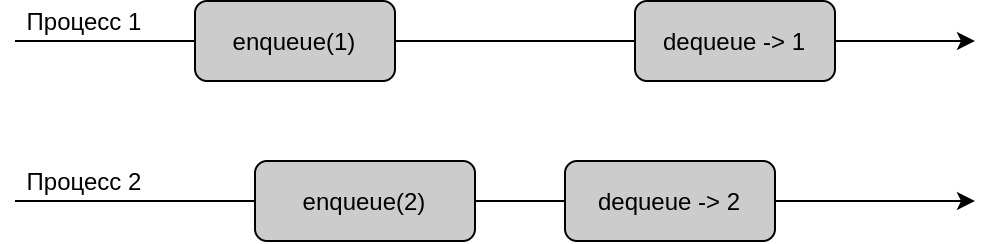
\includegraphics[scale=0.4]{NonSequential.jpg}
\end{figure}
В данном случае нарушается требование существования исполнения на одном процессе, в котором операция \textit{dequeue} вернула бы единицу дважды. \par
Однако подобные исполнения: 

\begin{figure}[h]
\caption{Последовательно согласованное исполнение}
\label{fig:sequential}
\vspace{2mm}
\centering
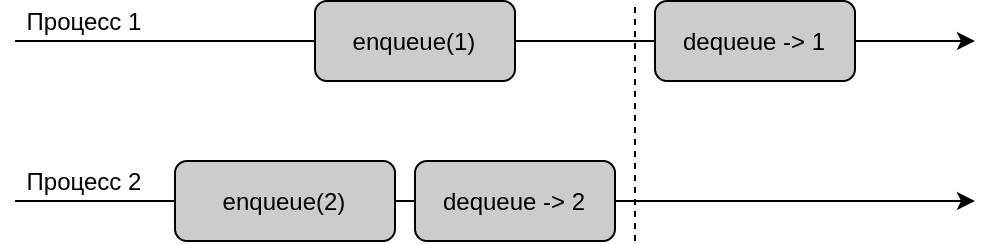
\includegraphics[scale=0.4]{Sequential.jpg}
\end{figure}
\noindentдопускаются, так как в данном случае все операции можно упорядочить в линейную историю, которая подчиняется спецификации объекта и сохраняет относительный порядок операций каждого из процессов:
\begin{figure}[h]
\caption{Объясняющее последовательное исполнение}
\label{fig:sequentialExpl}
\vspace{2mm}
\centering
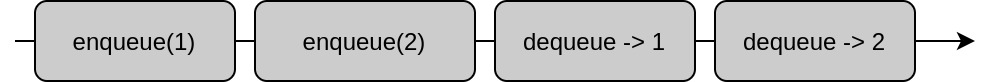
\includegraphics[scale=0.4]{SequentialExpl.jpg}
\end{figure}

Корректность конкурентного исполнения, приведенного на рисунке \ref{fig:sequential}, может показаться контр-интуитивной, поскольку операция \textit{dequeue -> 2} завершилась раньше, чем началась операция \textit{dequeue -> 1}, в отличие от объясняющего последовательного исполнения на рисунке \ref{fig:sequentialExpl}. \par
Также стоит отметить, что результат композиции последовательно согласованных объектов может не являться последовательно согласованным. Рассмотрим некоторую конкурентную историю для двух очередей \textit{Q1} и \textit{Q2}:

\begin{figure}[h]
\caption{Композиция последовательно согласованных объектов}
\vspace{2mm}
\centering
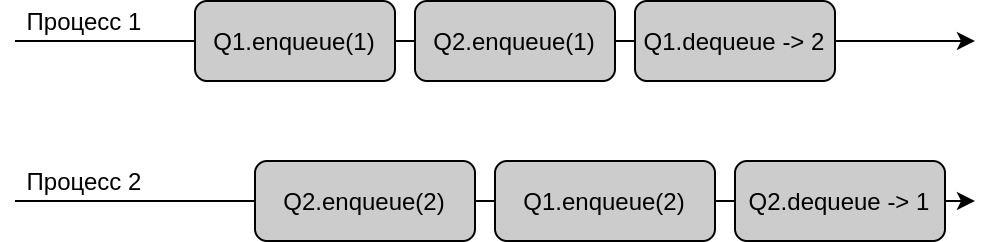
\includegraphics[scale=0.4]{SequentialComp.jpg}
\end{figure}
\noindent Для каждой из очередей по отдельности можно составить объясняющие последовательные истории, однако для всего исполнения в данном случае этого сделать нельзя. \par
Более строгой моделью согласованности, которая учитывает временной порядок операций, а также обладает свойством композиции, является \textit{линеаризуемость}. 

\subsection{Линеаризуемость}
Конкурентное исполнение называется \textit{линеаризуемым} (англ. \textit{linearizable}), если существует корректное с точки зрения спецификации последовательное исполнение, в котором сохранен относительный порядок не пересекающихся во времени операций. Участок кода называют линеаризуемым, если в нем не возможны состояния взаимной блокировки, и все его конкурентные исполнения линеаризуемы. Поскольку операции, исполняемые одним и тем же процессом, не пересекаются во времени, линеаризуемость подразумевает последовательную согласованность и является более сильным свойством. \cite{linearizable} \par
Согласно определению, последовательно согласованное исполнение, изображенное на рисунке \ref{fig:sequential}, не является линеаризуемым, поскольку не существует последовательной истории, которая одновременно и удовлетворяла бы спецификации ``первый пришел -- первый ушел'', и сохраняла бы порядок непересекающихся во времени операций \textit{dequeue -> 2} и \textit{dequeue -> 1}.\par
Однако конкурентные операции по-прежнему могут быть упорядочены произвольным образом в объясняющем последовательном исполнении, поэтому такое исполнение линеаризуемо:

\begin{figure}[h]
\caption{Линеаризуемое исполнение}
\vspace{2mm}
\centering
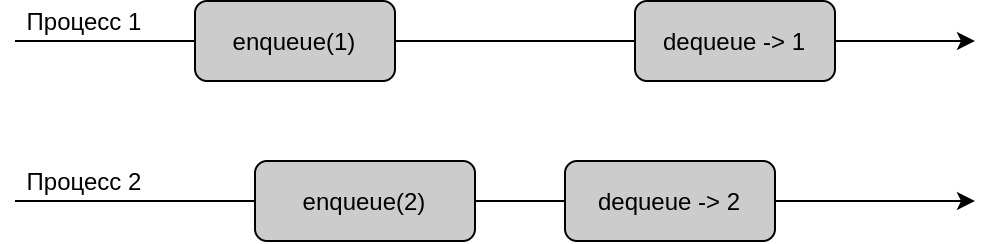
\includegraphics[scale=0.4]{Linearizable.jpg}
\end{figure}
\noindent Его линеаризация приведена на рисунке \ref{fig:sequentialExpl}\par

Линеаризуемость, в отличие от последовательной согласованности, является композирующимся свойством. \cite{linearizable} Это означает, что любое конкурентное исполнение кода, состоящего из операций над некоторыми объектами (например, структурами данных)  линеаризуемо, если и только если каждый из этих объектов линеаризуем по отдельности. Это свойство очень полезно, так как позволяет выделять некоторые ``строительные блоки'', облегчая рассуждения о поведении более сложных участков кода в конкурентной среде. \par
Данная работа фокусируется на рассмотрении последовательной согласованности и линеаризуемости, поскольку это наиболее часто используемые свойства. Однако стоит отметить, что существуют и применяются на практике и другие модели согласованности, такие как \textit{статическая} (англ. 
\textit{quiscent}) консистентность \cite{quiscent}, \textit{причинная} (англ. \textit{causal}) консистентность \cite{causal} и \textit{квази-линеаризуемость} (англ. \textit{quasi-linearizability}) \cite{quasi}.

\chapter{Проверка моделей согласованности}
В предыдущей главе мы рассмотрели некоторые удобные свойства, которые помогают рассуждать о поведении кода в многопроцессорных системах. Однако утверждения о том, что конкретные реализации структур данных обладают этими свойствами, нуждаются в проверке. Здесь можно выделить два основных подхода: 
\begin{itemize}
    \item \emph{Формальная проверка} (англ. \emph{verification}). Данный подход заключается в предоставлении доказательства корректности конкретного кода при фиксированной модели памяти. Это самый надежный подход из существующих, однако эта проблема решена лишь для некоторых классов задач и требует значительных усилий \cite{seqVerification}. Например, решения для проверки на линеаризуемость основаны на поиске точек линеаризации \cite{linVerification}. Однако в некоторых структурах данных точек линеаризации не существует \cite{linearizable}. Статический анализ кода, отсутствие универсальности и требование знаний о моделях памяти, теории моделей согласованности и методов верификации делает затруднительным широкое применение этого подхода.
    \item \emph{Тестирование} (англ. \emph{model checking}). Представляет из себя перебор возможных исполнений программы и последующую проверку результатов исполнения относительно последовательной спецификации. Это не может гарантировать корректность проверяемого кода, однако не требует глубокого анализа и хорошо работает на практике, находя большое количество ошибок. \cite{lineup} 
\end{itemize}

В данной главе мы сосредоточимся на алгоритмах тестирования конкурентных структур данных на соответствие моделям последовательной согласованности и линеаризуемости, а также разработаем набор требований для библиотеки, реализующей данный функционал.

\section{Постановка задачи}
Пусть есть некоторая реализация конкурентной структуры данных. Обозначим количество доступных в ней операций через \(M\). Пусть каждый из \(T\) конкурентных потоков совершает по \(L\) операций. Тогда количество возможных конкурентных сценариев исполнения без учета симметрии равно
\((C_M^L)^T\), где \(C_M^L\) -- количество способов составить сценарий исполнения для одного потока. \par
Кроме того, результаты запусков каждого из сценариев будут различны из-за отсутствия каких-либо гарантий от планировщика задач. При этом для каждого запуска некоторого сценария еще необходимо проверить, удовлетворяет ли он заявленной модели согласованности. Как для последовательной согласованности, так и для линеаризуемости эта задача является NP-полной \cite{complexity}. \par
Стремительный рост пространства состояний, а также неподконтрольность системного планировщика делает невозможным проверку абсолютно всех возможных ситуаций. Однако на практике это и не требуется. Опыт показывает, что для обнаружения всех известных ошибок обычно достаточно проводить тестирования на двух-трех конкурентных процессах со сценариями, не превосходящими по длине пяти-десяти операций \cite{lineup}.

\section{Алгоритмы тестирования}
Для проверки последовательной согласованности и, в особенности, линеаризуемости было предложено множество алгоритмов \cite{checkAlgorithms}. В данном разделе мы остановимся на простейших из них. \par
У алгоритмов проверки обоих моделей можно выделить общую часть, которая будет различаться лишь реализацией функции \textit{possibleOperations}: 
\lstinputlisting[language=Scala, 
caption=Общий алгоритм проверки
]{Common.pseudo}
Прокомментируем алгоритм построчно:
\begin{itemize}
    \item \emph{Строка 1} -- на вход алгоритм принимает \emph{history} - историю конкурентного исполнения, включающая информацию о всех вызванных операциях и их результатах, а также \emph{state} - реализацию тестируемой структуры данных с возможностью ``отмены'' операций (о способах реализации отмены мы поговорим позднее).
    \item \emph{Строка 2} -- пустая история всегда корректна.
    \item \emph{Строки 3-4} -- если история не пуста, то начать перебор всех допустимых операций конкурентного исполнения, которые могли бы стать следующими в объясняющей последовательной истории. Вычисление этого списка кандидатов в методе \emph{possibleOperatoins} зависит от проверяемой модели согласованности.
    \item \emph{Строка 5} -- обозначаем результат исполнения рассматриваемой операции-кандидата за \emph{res}.
    \item \emph{Строки 6-11} -- применяем рассматриваемую операцию к \emph{state}. Если результат исполнения операции совпал с \emph{res}, продолжаем проверку корректности для оставшейся истории. Если проверка для оставшейся истории успешна, то сообщаем, что \emph{history} корректна с точки зрения выбранной модели согласованности.
    \item \emph{Строка 13} -- сообщаем, что \emph{history} не является корректной, поскольку не нашлось объясняющих ее последовательных исполнений.
\end{itemize}
\subsection{Последовательная согласованность}
В случае последовательной согласованности функция \emph{possibleOperations} реализуется как список следующих по очереди операций каждого из процессов в программном порядке:
\lstinputlisting[language=Scala,
caption=Поиск операций-кандидатов для последовательной согласованности
]{Sequential.pseudo}

\subsection{Линеаризуемость}
Для линеаризуемости помимо программного порядка необходимо учитывать также и временной порядок операций, поэтому реализация функции \emph{possibleOperations} отличается:
\lstinputlisting[language=Scala,
caption=Поиск операций-кандидатов для линеаризуемости
]{Linearizable.pseudo}

\section{Разработка требований к библиотеке}

\subsection{Интерфейс}

\subsection{Конфигурация}

\chapter{Реализация библиотеки}

\section{Интерфейс}

\section{Генерация тестовых сценариев}

\section{Запуск тестовых сценариев}

\section{Валидация результатов исполнения}

\section{Генерация отчета тестирования}

\chapter{Выводы}

\bibliographystyle{unsrt}
\bibliography{references}

\end{document}

